%% Copyright 2019-2021 Elsevier Ltd
%% 
%% This file is part of the 'CAS Bundle'.
%% --------------------------------------
%% 
%% It may be distributed under the conditions of the LaTeX Project Public
%% License, either version 1.2 of this license or (at your option) any
%% later version.  The latest version of this license is in
%%    http://www.latex-project.org/lppl.txt
%% and version 1.2 or later is part of all distributions of LaTeX
%% version 1999/12/01 or later.
%% 
%% The list of all files belonging to the 'CAS Bundle' is
%% given in the file `manifest.txt'.
%% 
%% Template article for cas-sc documentclass for 
%% single column output.

\documentclass[a4paper,fleqn]{cas-sc}

% If the frontmatter runs over more than one page
% use the longmktitle option.

%\documentclass[a4paper,fleqn,longmktitle]{cas-sc}

%\usepackage[numbers]{natbib}
%\usepackage[authoryear]{natbib}
\usepackage[authoryear,longnamesfirst]{natbib}

%%%Author macros
\def\tsc#1{\csdef{#1}{\textsc{\lowercase{#1}}\xspace}}
\tsc{WGM}
\tsc{QE}
%%%

% Uncomment and use as if needed
%\newtheorem{theorem}{Theorem}
%\newtheorem{lemma}[theorem]{Lemma}
%\newdefinition{rmk}{Remark}
%\newproof{pf}{Proof}
%\newproof{pot}{Proof of Theorem \ref{thm}}

\begin{document}
\let\WriteBookmarks\relax
\def\floatpagepagefraction{1}
\def\textpagefraction{.001}

% Short title
\shorttitle{Machine Learning wave prediction with Spectra}    

% Short author
\shortauthors{LPeach, NCartwright, GVieraDeSilva}  

% Main title of the paper
\title [mode = title]{Machine Learning wave prediction using spectra}  

% Title footnote mark
% eg: \tnotemark[1]
\tnotemark[<tnote number>] 

% Title footnote 1.
% eg: \tnotetext[1]{Title footnote text}
\tnotetext[<tnote number>]{<tnote text>} 

% First author
%
% Options: Use if required
% eg: \author[1,3]{Author Name}[type=editor,
%       style=chinese,
%       auid=000,
%       bioid=1,
%       prefix=Sir,
%       orcid=0000-0000-0000-0000,
%       facebook=<facebook id>,
%       twitter=<twitter id>,
%       linkedin=<linkedin id>,
%       gplus=<gplus id>]

\author[<aff no>]{Leo Peach}

% Corresponding author indication
\cormark[<corr mark no>]

% Footnote of the first author
\fnmark[<footnote mark no>]

% Email id of the first author
\ead{leo.peach@griffithuni.edu.au}

% URL of the first author
\ead[url]{<URL>}

% Credit authorship
% eg: \credit{Conceptualization of this study, Methodology, Software}
\credit{Methodology, Scientific writing, literature review, software}

% Address/affiliation
\affiliation[<aff no>]{organization={Griffith University},
            addressline={Southport}, 
            city={Gold Coast},
%          citysep={}, % Uncomment if no comma needed between city and postcode
            postcode={0000}, 
            state={Queensland},
            country={Australia}}

\author[<aff no>]{Leo Peach}

% Footnote of the second author
\fnmark[2]

% Email id of the second author
\ead{}

% URL of the second author
\ead[url]{}

% Credit authorship
\credit{Leo Peach}

% Address/affiliation
\affiliation[<aff no>]{organization={Griffith University},
            addressline={Southport}, 
            city={Gold Coast},
%          citysep={}, % Uncomment if no comma needed between city and postcode
            postcode={00000}, 
            state={Queensland},
            country={Australia}}

% Corresponding author text
\cortext[1]{Leo Peach}

% Footnote text
\fntext[1]{}

% For a title note without a number/mark
%\nonumnote{}
% Here goes the abstract
\begin{abstract}
Here we describe a method for improving predicting using a 1D wave spectrum.
\end{abstract}

% Use if graphical abstract is present
%\begin{graphicalabstract}
%\includegraphics{}
%\end{graphicalabstract}

% Research highlights
\begin{highlights}
\item Machine Learning
\item Wave Prediction
\item Spectra
\end{highlights}

% Keywords
% Each keyword is seperated by \sep
\begin{keywords}
Machine Learning \sep Wave Prediction \sep Spectra
\end{keywords}

%\maketitle

% Main text
\section{Introduction}\label{Intro}
The forecasting of wave heights is important for a range of maritime and coastal applications, from port operations through to beach management and surfing. One of the challenges is the ability to downscale predictions from oceanographic wave models to the coast. This is required as additional physical processes occur as the waves approach local features, such as depth induced wave breaking, refraction and defraction. Typically this involves the development of computationally expensive physics based models, which also require good quality input data, including bathymetry to perform well.
Data-driven approaches have increasingly been applied in order to help overcome the computational cost and allow the rapid downscaling of wave forecasts and hindcasts. Most have utilised wave parameters <<<<REFS HERE>>>> , but this can have it's challenges as wave parameters are summaries of the wave spectrum (which is a more full description of wave conditions in the form of energy spread over a range of frequencies)<<<REFS>>>. 
Machine learning techniques are being increasingly applied in this space


\section{Method}\label{method}

\subsection{Datasets}
Training of the machine learning models can require a substantial amount of data, two key datasets were used for training. Offshore wave spectrum from a wave watch 3 model (in this case the CAWCR wave hindcast) and wave observations at the point of interest. The CAWCR wave hindcast spectrum consists of a 2d dimensional wave spectrum with 30 directional bins and X frequency bins at y spacing.

% Figure
\begin{figure}[<options>]
	\centering
		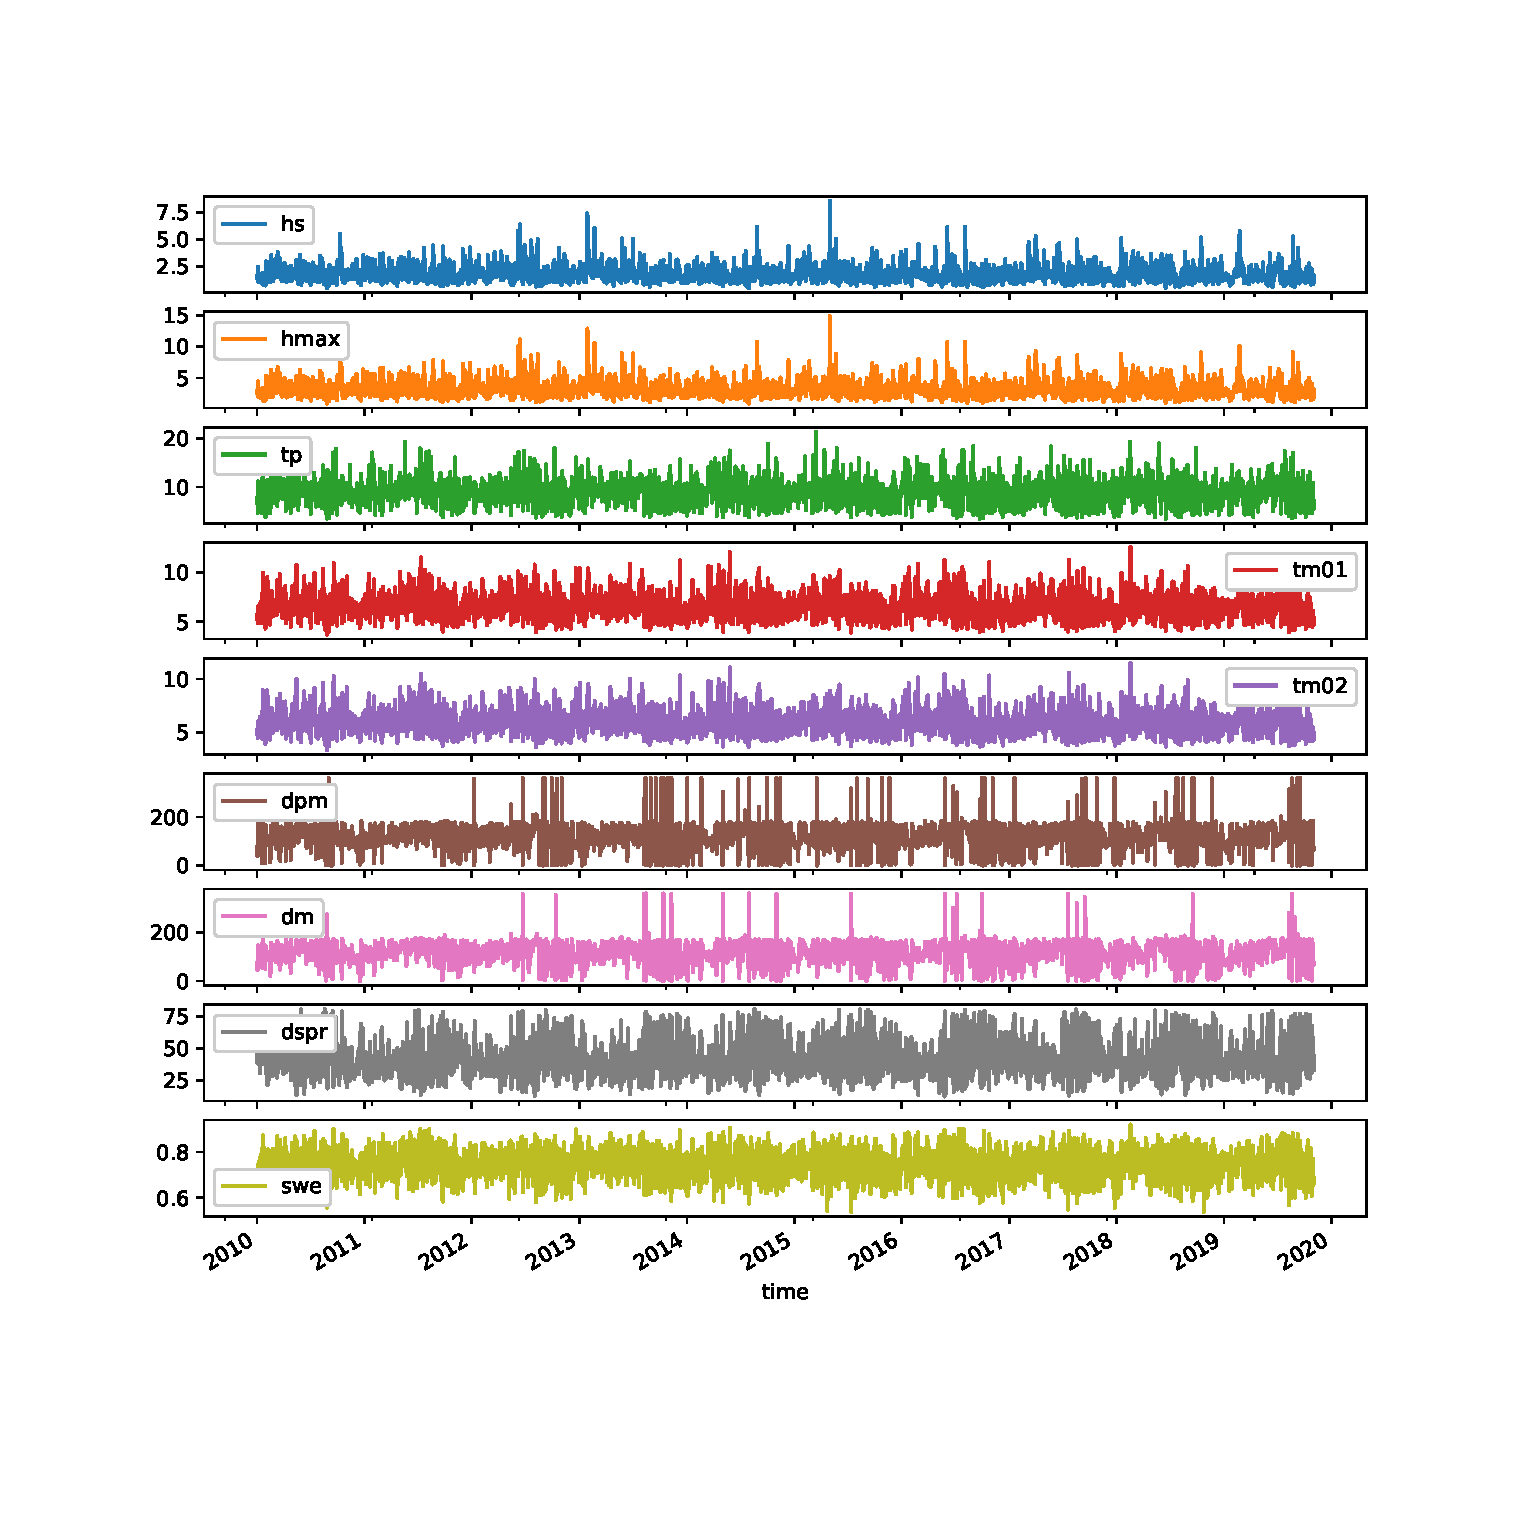
\includegraphics[<options>]{'../notebooks/offshore_modelled.eps'}
	  \caption{}\label{fig1}
\end{figure}

Wave observations sourced from the Queensland Government Wave Monitoring program for sites shown in figure 4. The length of the wave monitoring data for each site was varied and training was therefore undertaken on the available data.

\subsubsection{Data preparation}
Extracting features from training data is key element in training machine learning models. As well as extracting features each dataset needed to be cleaned to ensure consistency, remove errors and fill gaps where possible. 

To simplify the 2 dimensional wave spectrum for each of the offshore points two processing steps were undertaken, first wave parameters were extracted, second the spectrum was integrated into a 1 dimensional spectrum (integrating directions together). Wave parameters calculated including, Tp, pDir, Hs, Tz and zDir. Directional values were split into x and y values.

The wave monitoring data also required a range of pre-processing techniques, as the data is based on observational equipment there were several issues present in the dataset. These included error values, small data gaps, large data gaps and spurious values. Error values were removed, small gaps (< 3 hours) were linearly interpolated and spurious data was removed using a range filter. Directional values were converted into x and y values. 

The datasets were then merged to create a continuous dataset, and for feature extraction. Features were then extracted, particularly focussed on identifying seasonality in the time series data, months, days, year and hours were all added to the training dataset. 

\subsection{Training, Testing, Validation}
The dataset was split into validation (~1 year of data) with testing and training each being 80\% and 20\% of the remainder. Scaling was undertaken on the entire dataset to ensure that scaled data included all the data within the minimum and maximum of the dataset. 
Time series cross validation was configured for model training, with a growing training window of 7 days.

\section{Machine Learning Model}
An Long-Term Short-Term memory model was selected....

\section{Discussion}\label{disc}


\section{Conclusion}\label{con}


% Numbered list
% Use the style of numbering in square brackets.
% If nothing is used, default style will be taken.
%\begin{enumerate}[a)]
%\item 
%\item 
%\item 
%\end{enumerate}  

% Unnumbered list
%\begin{itemize}
%\item 
%\item 
%\item 
%\end{itemize}  

% Description list
%\begin{description}
%\item[]
%\item[] 
%\item[] 
%\end{description}  

% Figure
%\begin{figure}[<options>]
%	\centering
%		\includegraphics[<options>]{}
%	  \caption{}\label{fig1}
%\end{figure}


%\begin{table}[<options>]
%\caption{}\label{tbl1}
%\begin{tabular*}{\tblwidth}{@{}LL@{}}
%\toprule
%  &  \\ % Table header row
%\midrule
% & \\
% & \\
% & \\
% & \\
%\bottomrule
%\end{tabular*}
%\end{table}

% Uncomment and use as the case may be
%\begin{theorem} 
%\end{theorem}

% Uncomment and use as the case may be
%\begin{lemma} 
%\end{lemma}

%% The Appendices part is started with the command \appendix;
%% appendix sections are then done as normal sections
%% \appendix

\section{}\label{}

% To print the credit authorship contribution details
%\printcredits

%% Loading bibliography style file
%\bibliographystyle{model1-num-names}
\bibliographystyle{cas-model2-names}

% Loading bibliography database
\bibliography{}

% Biography
\bio{}
Leo is a PhD candidate at the Griffith Univeristy School of Engineering and Built Environment, and the Marine and Coastal Research Centre
\endbio

%\bio{}
%% Here goes the biography details.
%\endbio

\end{document}

